\documentclass[12pt]{beamer}
\usetheme{Boadilla}
\usepackage{booktabs}
\usepackage{multirow}
\usepackage{enumitem}
\usepackage{tikz}

\newcommand{\E}{\mathbb{E}}
\usefonttheme{professionalfonts}
\usepackage{pgfplots}
\pgfplotsset{compat=1.18}
\renewcommand{\arraystretch}{1.25}
\usetikzlibrary{trees}
\title[ECON2843]{Lecture 22}
\subtitle{Part 5 Linear Regression}
\date{}
\usepackage{amsmath,amssymb,mathtools,wasysym}
\begin{document}
	\begin{frame}
		\titlepage
		
	\end{frame}
	\begin{frame}
		\vspace{1cm}
		\centering
		{\color{blue}\large Simple Linear Regression}
	\end{frame}


	\begin{frame}
		\frametitle{\color{blue}Simple Linear Regression}
		
		\vspace{1cm}
		
		\begin{itemize}[label={\color{blue}$\blacktriangleright$}]
			\item Simple linear regression is used to investigate the relationship between two variables, denoted $X$ and $Y$.
			
			\vspace{0.5cm}
			
			\item $X$ is called the \textbf{independent}, \textbf{explanatory}, \textbf{predictor} or \textbf{regressor} variable.
			
			\vspace{0.5cm}
			
			\item $Y$ is called the \textbf{dependent} or \textbf{response} variable.
		\end{itemize}
		
	\end{frame}
\begin{frame}
	\frametitle{\color{blue}Simple Linear Regression}
	
	
	\begin{itemize}[label={\color{blue}$\blacktriangleright$}]
		\item Simple linear regression can be used to:
	\end{itemize}
	
	\begin{enumerate}[label={\color{blue}\arabic{enumi}}.]
		\item Determine whether there is a linear relationship between $X$ and $Y$ (does the value of $X$ have any effect on the value of $Y$?).
		
		\item Determine the nature of the linear relationship between $X$ and $Y$ (as $X$ changes, how does $Y$ change?).
		
		\item {\color{red}Predict the value of $Y$ from a value of $X$.}
	\end{enumerate}
	
\end{frame}
\begin{frame}
	\frametitle{\color{blue}Simple Linear Regression}
	
	
	\begin{itemize}[label={\color{blue}$\blacktriangleright$}]
		\item $X$ and $Y$ are both usually continuous variables.
		
		\item However, we will consider situations in multiple regression that involve categorical independent variables.
		
		\item Note: Multiple regression (more on this next topic) refers to when there is more than one independent variable, i.e., $X_1, X_2, X_3, \ldots$
	\end{itemize}
	
\end{frame}
\begin{frame}
	\frametitle{\color{blue}Example}
	
	
	\begin{itemize}[label={\color{blue}$\blacktriangleright$}]
		\item Suppose we want to use simple linear regression to see whether the time a person has lived in a city affects their attitude toward that city in a linear manner.
		
		\item Since we want to see how attitude is affected by duration of residence, we would set:
		\begin{itemize}[label={\color{blue}$\blacktriangleright$}]
			\item Duration of residence as the independent variable $X$.
			\item Attitude toward the city as the dependent variable $Y$.
		\end{itemize}
	\end{itemize}
	
\end{frame}
\begin{frame}
	\frametitle{\color{blue}Example}
	
	
	\begin{itemize}[label={\color{blue}$\blacktriangleright$}]
		\item Let our sample data be denoted by the pairs of values $\{(X_1, Y_1),\ldots,(X_n, Y_n)\}$.
		
		\item Now, the first step in conducting a simple linear regression analysis is to construct a scatter plot so we can ``eyeball'' the data.
		
		\item Plot the independent variable $X$ on the $x$-axis and dependent variable $Y$ on the $y$-axis.
	\end{itemize}
	
\end{frame}
\begin{frame}
	\frametitle{Scatter Plot}
	\centering
	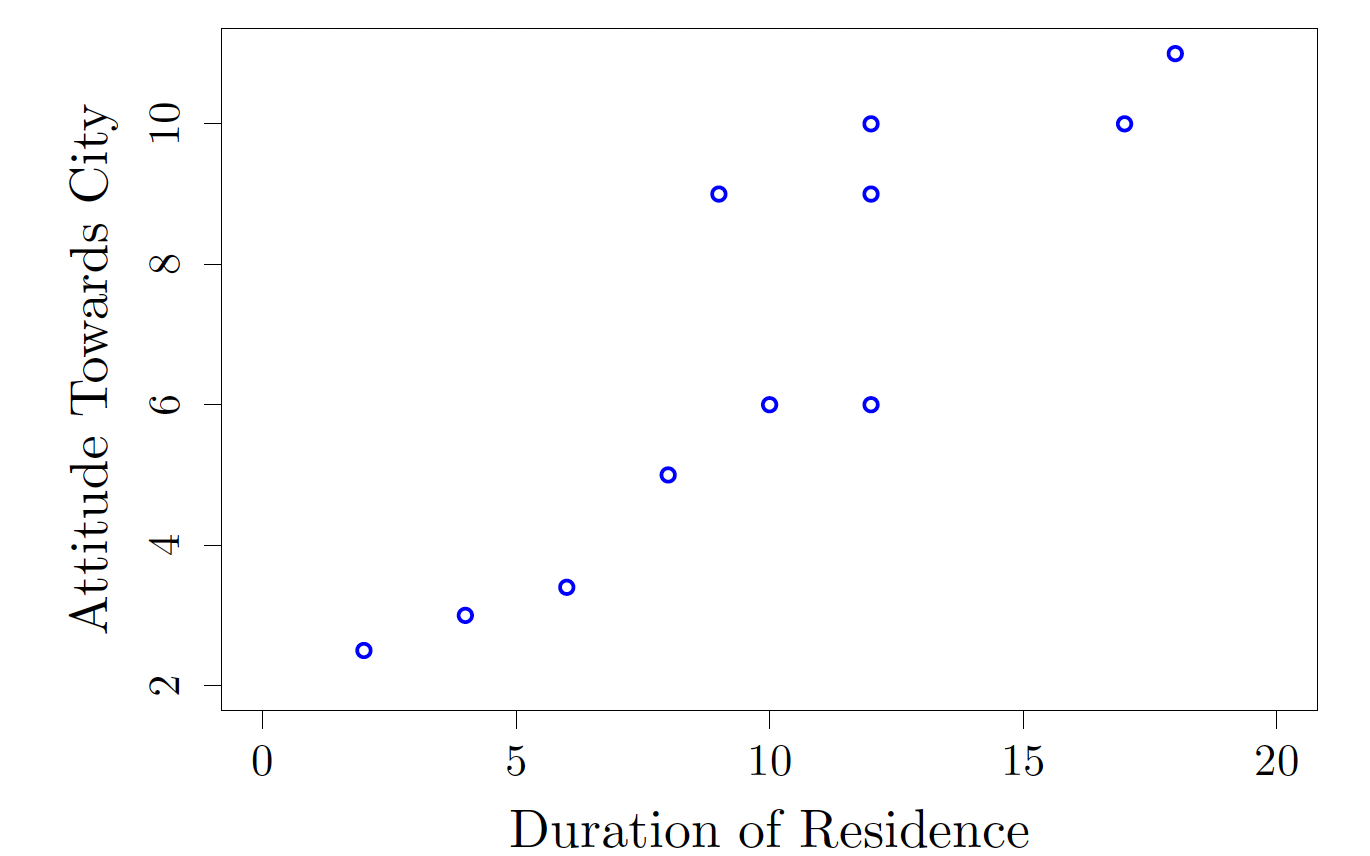
\includegraphics[width=12cm]{scatter.png}
	
\end{frame}
\begin{frame}
	\frametitle{\color{blue}Simple Linear Regression Model}
	
	
	\begin{itemize}[label={\color{blue}$\blacktriangleright$}]
		\item The \textbf{simple linear regression model} assumes that the relationship between the dependent and independent variables is given by a straight line:
		
		\[Y = \beta_0 + \beta_1X + \epsilon\]
		
		\item $\beta_0$ is the $y$-intercept of the line.
		
		\item $\beta_1$ is the slope of the line.
		
		\item $\epsilon$ is called the error variable.
	\end{itemize}
	
\end{frame}
\begin{frame}
	\frametitle{\color{blue}Simple Linear Regression Model}
	
	
	\begin{itemize}[label={\color{blue}$\blacktriangleright$}]
		\item In our city example, if we took the $i$th person from our sample with duration of residence $X_i$ and attitude $Y_i$, then the simple linear regression model states that:
		
		\[Y_i = \beta_0 + \beta_1X_i + \epsilon_i\]
		
		\item That is, their attitude $Y_i$ is equal to $\beta_0 + \beta_1X_i$ plus some amount $\epsilon_i$.
		
		\item The amount $\epsilon_i$ signifies a random error component that can be either positive, negative or zero.
	\end{itemize}

\end{frame}
\begin{frame}
	\frametitle{Simple Linear Regression Model}
	\centering
	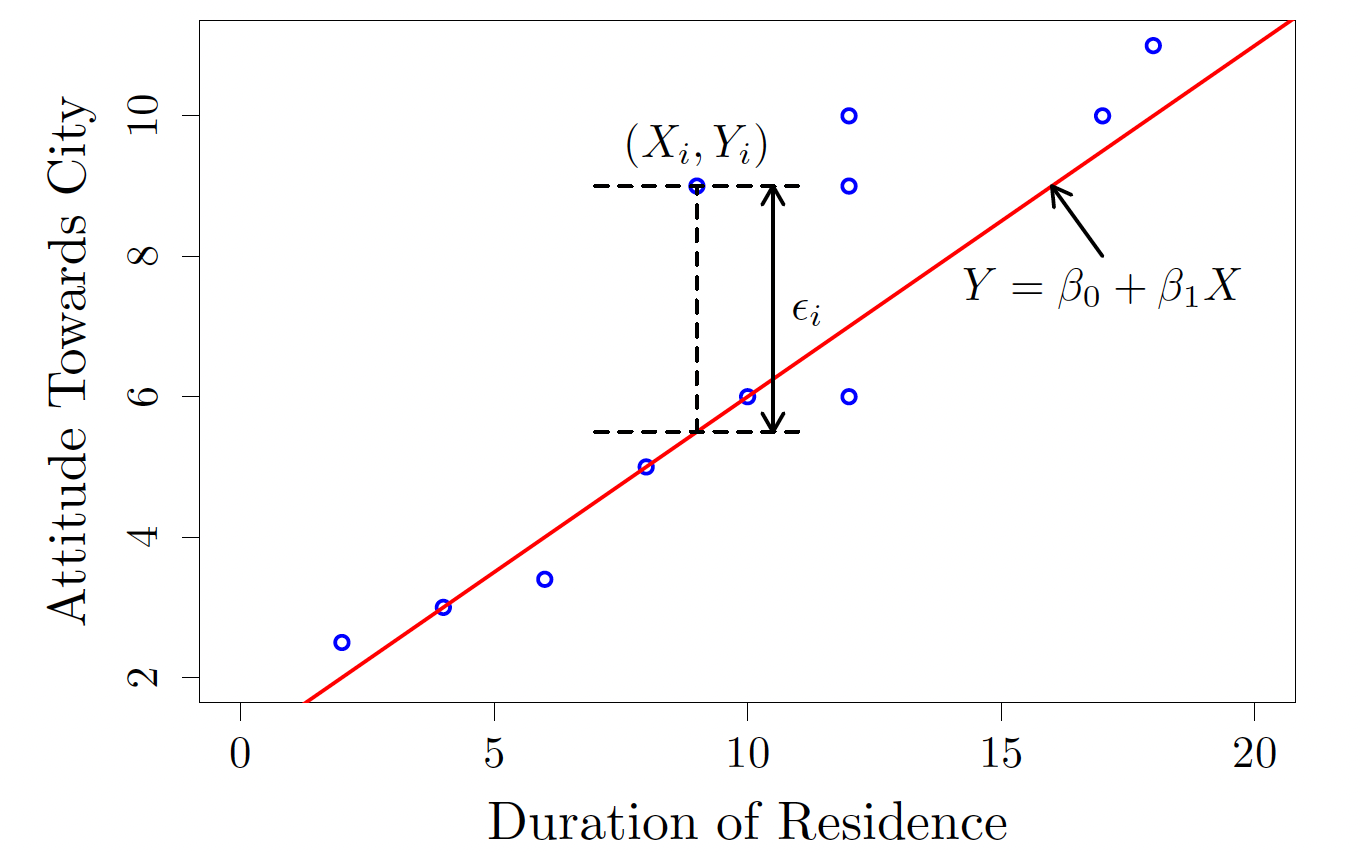
\includegraphics[width=12cm]{simple.png}
	
\end{frame}
\begin{frame}
	\frametitle{\color{blue}Model Assumptions}
	
	\begin{itemize}[label={\color{blue}$\blacktriangleright$}]
		\item As was the case with ANOVA, the simple linear regression model makes a number of assumptions and these are stated in terms of the error variable $\epsilon$.
		
		\item The assumptions are that the errors:
		\begin{itemize}[label={\color{blue}$\blacktriangleright$}]
			\item Are normally distributed.
			\item Have mean equal to 0.
			\item Have constant variance denoted by $\sigma_\epsilon^2$, regardless of the value of $X$.
			\item Are independent.
		\end{itemize}
		
		\item Shorthand we write $\epsilon_i \stackrel{iid}{\sim} N(0,\sigma_\epsilon^2)$.
		\begin{itemize}[label={\color{blue}$\blacktriangleright$}]
			\item \textit{iid} stands for ``independently and identically distributed''.
		\end{itemize}
	\end{itemize}
	
\end{frame}
\begin{frame}
	\frametitle{\color{blue}The Error Variable $\epsilon$}
	
	
	\begin{itemize}[label={\color{blue}$\blacktriangleright$}]
		\item Why is there an error variable?
		
		\item Suppose you take two observations from the population with the same value of $X$.
		
		\item Will they have the same value of $Y$?
		
		\item Probably not. Why?
		
		\item Because of the inherent variability in the population.
	\end{itemize}
	
\end{frame}
\begin{frame}
	\frametitle{\color{blue}The Error Variable $\epsilon$}
	
	
	\begin{itemize}[label={\color{blue}$\blacktriangleright$}]
		\item The error variable represents this inherent variability that exists in the population.
		
		\item In fact, if we look at \textit{all} the observations in the population that have a particular value of $X = x^*$, due to this inherent variability, there will be a corresponding distribution of $Y$ values.
	\end{itemize}
	
\end{frame}
\begin{frame}
	\frametitle{\color{blue}The Error Variable $\epsilon$}
	\centering
	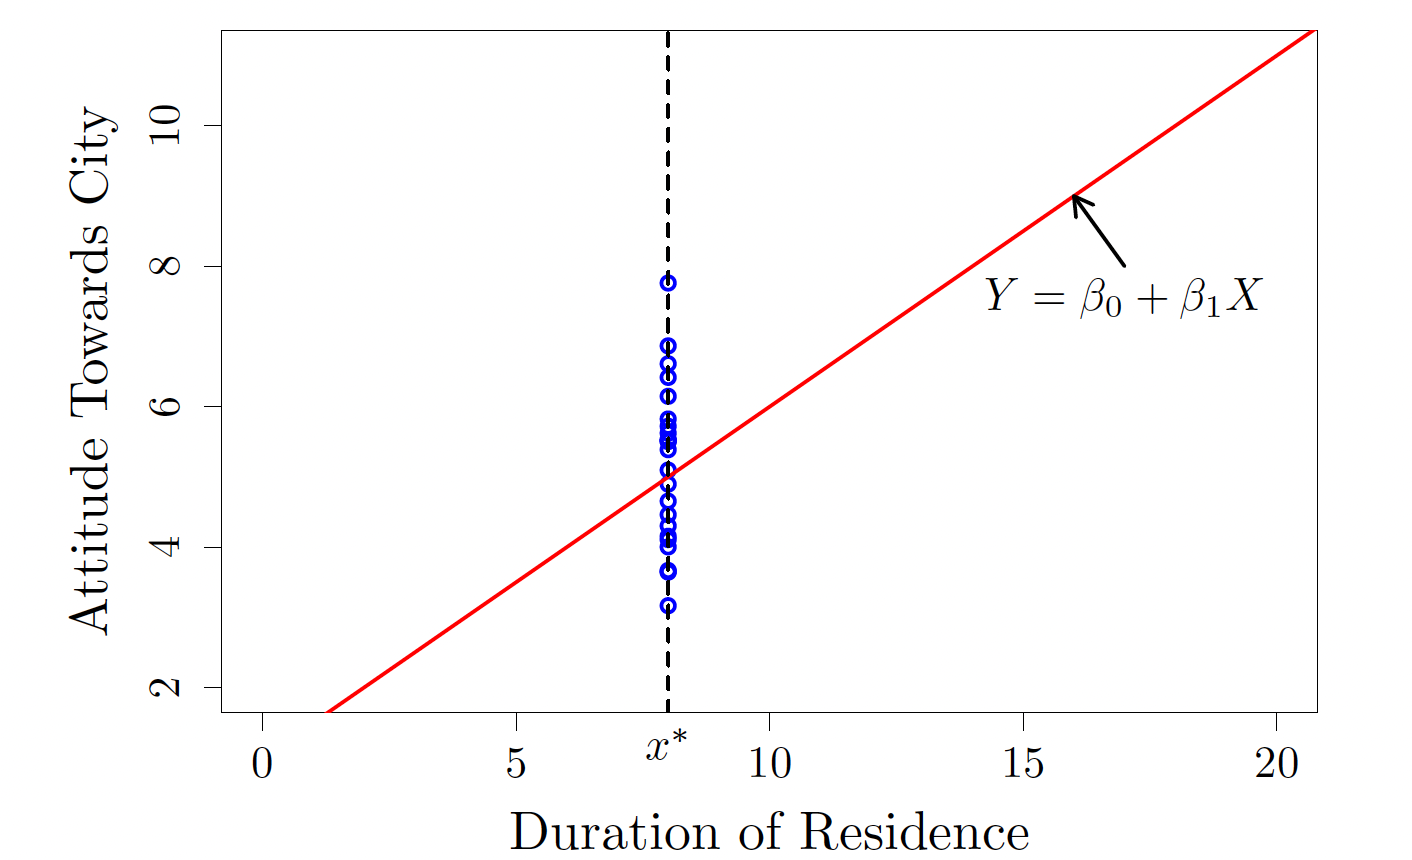
\includegraphics[width=12cm]{error.png}
	
\end{frame}
\begin{frame}
	\frametitle{\color{blue}The Error Variable $\epsilon$}
	\centering
	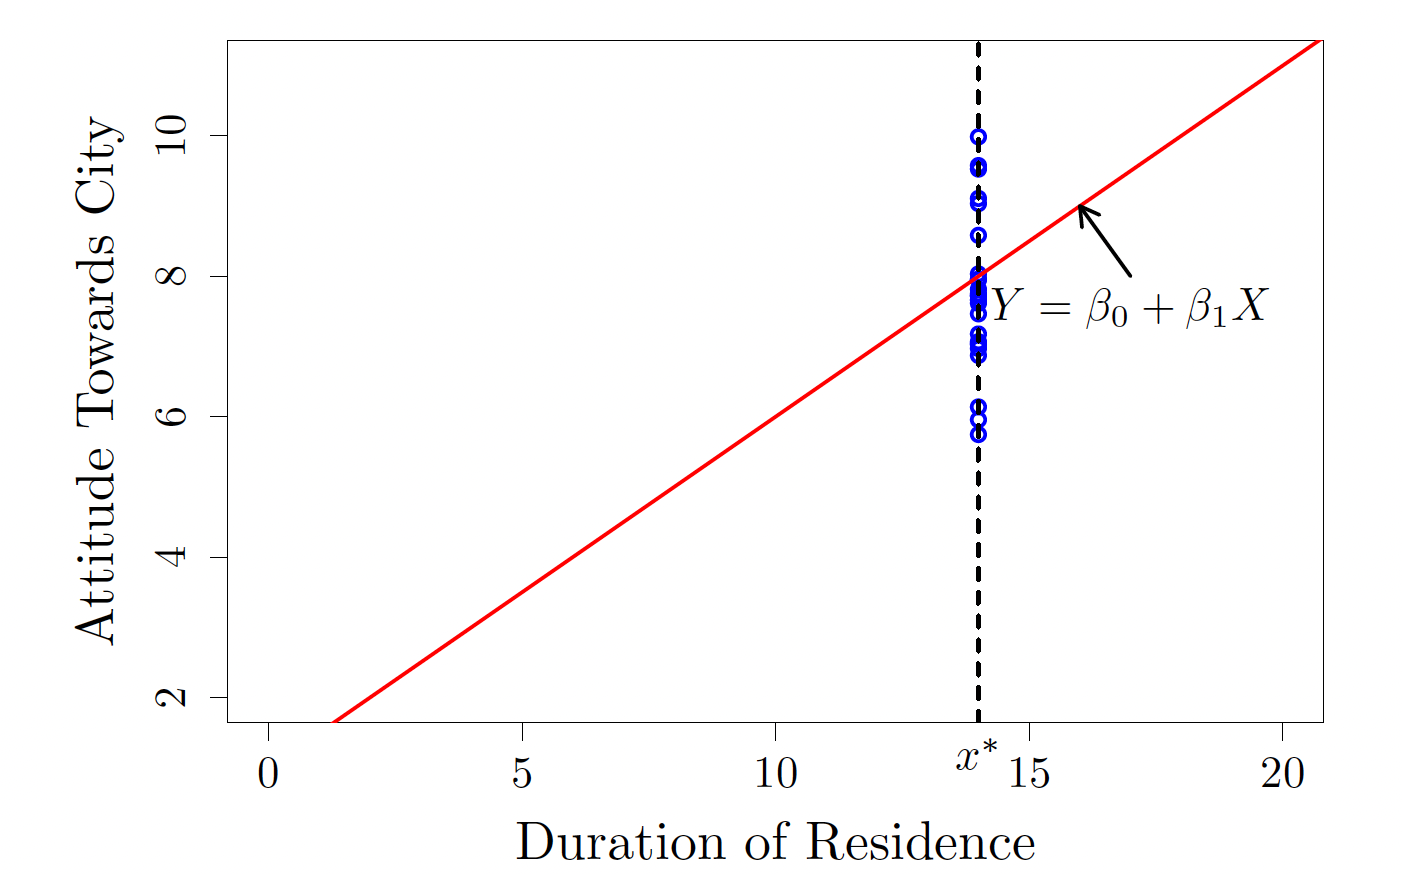
\includegraphics[width=12cm]{error2.png}
	
\end{frame}
\begin{frame}
	\frametitle{The Error Variable $\epsilon$}
	
	\begin{itemize}[label={\color{blue}$\blacktriangleright$}]
		\item Based on the model assumptions, the distribution of the $Y$ values given $X = x^*$ is actually normal with mean and variance given by:

	\end{itemize}
		\begin{align*}
		E(Y) &= E(\beta_0 + \beta_1x^* + \epsilon) \\
		&= \beta_0 + \beta_1x^* + E(\epsilon) \\
		&= \beta_0 + \beta_1x^*
	\end{align*}
	
	\begin{align*}
		V(Y) &= V(\beta_0 + \beta_1x^* + \epsilon) \\
		&= V(\epsilon) \\
		&= \sigma_\epsilon^2
	\end{align*}
\end{frame}
\begin{frame}
	\frametitle{\textcolor{blue}{Simple Linear Regression Model}}
	
	\begin{itemize}[label={\color{blue}$\blacktriangleright$}]
		\item Therefore, another way to state the simple linear regression model is that the dependent variable $Y$ is normally distributed with mean equal to:
		
		\[
		E(Y) = \beta_0 + \beta_1X
		\]
		
		and variance equal to:
		
		\[
		V(Y) = \sigma_\epsilon^2
		\]
	\end{itemize}
	
\end{frame}
\begin{frame}
	\frametitle{\textcolor{blue}{Parameter Estimation}}
	
	\begin{itemize}[label={\color{blue}$\blacktriangleright$}]
		\item The intercept $\beta_0$ and slope $\beta_1$ of the simple linear regression model are unknown \textit{population parameters}.
		
		\item Therefore, to actually \textit{fit} the model, we need to \textit{estimate} $\beta_0$ and $\beta_1$.
		
		\item How do we do that? By using our sample data, $\{(X_1,Y_1),\ldots,(X_n,Y_n)\}$.
	\end{itemize}
	
\end{frame}

\begin{frame}
	\frametitle{\textcolor{blue}{Parameter Estimation}}
	
	\begin{itemize}[label={\color{blue}$\blacktriangleright$}]
		\item In other words, based on the observations in our sample, we are trying to find the best estimate of the straight line given by our model:
		
		\[
		Y = \beta_0 + \beta_1X
		\]
		
		\item Suppose we have somehow obtained estimates for $\beta_0$ and $\beta_1$, denoted by $\hat{\beta}_0$ and $\hat{\beta}_1$, respectively.
	\end{itemize}
	
\end{frame}
\begin{frame}
	\frametitle{\textcolor{blue}{Parameter Estimation}}
	
	\begin{itemize}[label={\color{blue}$\blacktriangleright$}]
		\item Then our \textbf{estimated} or \textbf{fitted regression line} is:
		
		\[
		\hat{Y} = \hat{\beta}_0 + \hat{\beta}_1X
		\]
		
		\item So for each observation in our sample, we can calculate its \textbf{fitted value}:
		
		\[
		\hat{Y}_i = \hat{\beta}_0 + \hat{\beta}_1X_i
		\]
	\end{itemize}
	
\end{frame}
\begin{frame}
	\frametitle{\textcolor{blue}{Parameter Estimation}}
	\centering
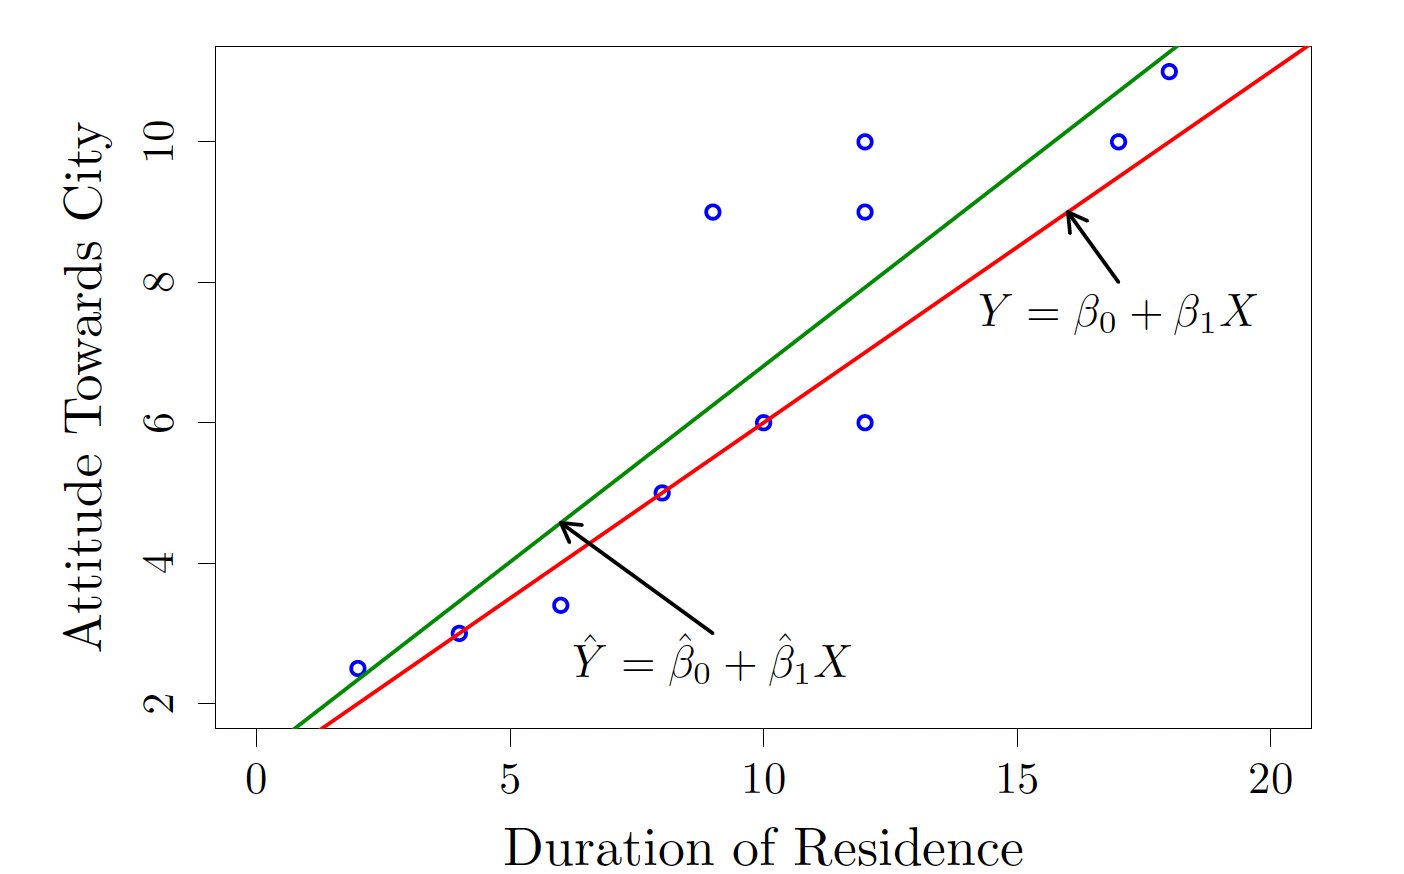
\includegraphics[width=12cm]{para.png}
\end{frame}
\begin{frame}
	\frametitle{\textcolor{blue}{Parameter Estimation}}
	\centering
	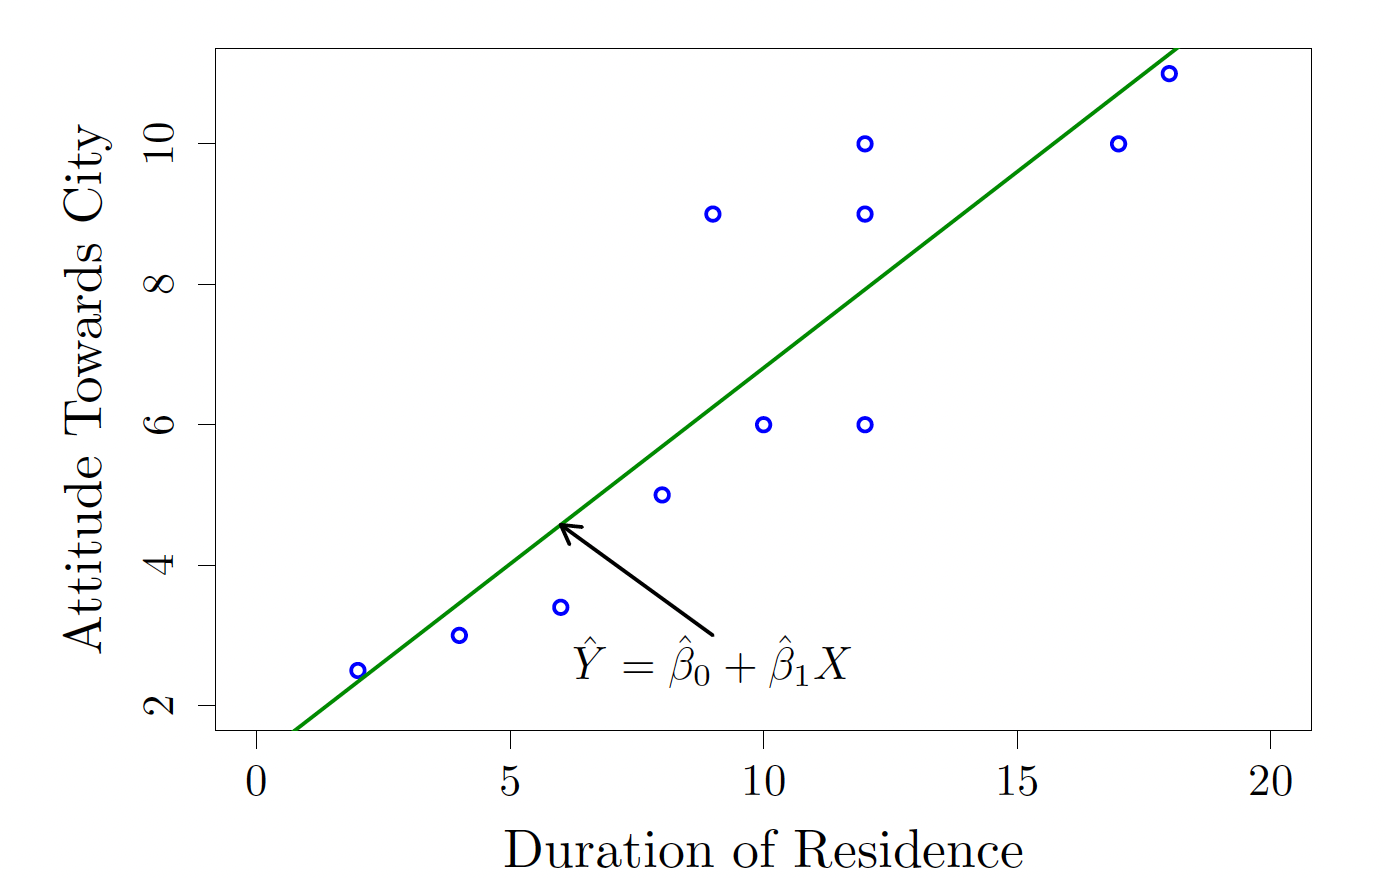
\includegraphics[width=12cm]{para2.png}
\end{frame}
\begin{frame}
	\frametitle{\textcolor{blue}{Parameter Estimation}}
	
	\begin{itemize}[label={\color{blue}$\blacktriangleright$}]
		\item Recall that, based on the simple linear regression model, the $Y_i$ value for each observation in our sample can be expressed as:
		
		\[
		Y_i = \beta_0 + \beta_1X_i + \epsilon_i
		\]
		
		\item We can do a similar thing based on\ldots
	\end{itemize}
	
\end{frame}
\begin{frame}
	\frametitle{\textcolor{blue}{Parameter Estimation}}
	
	\begin{itemize}[label={\color{blue}$\blacktriangleright$}]
		\item \ldots our \textit{fitted regression line}:
		
		\[
		Y_i = \hat{\beta}_0 + \hat{\beta}_1X_i + e_i
		\]
		
		\item The term $e_i$ is called the \textbf{residual} of the $i$th observation and is just equal to:
		
		\begin{align*}
			e_i &= Y_i - (\hat{\beta}_0 + \hat{\beta}_1X_i) \\
			&= Y_i - \hat{Y}_i
		\end{align*}
	\end{itemize}
	
\end{frame}
\begin{frame}
	\frametitle{\textcolor{blue}{Parameter Estimation}}
	\centering
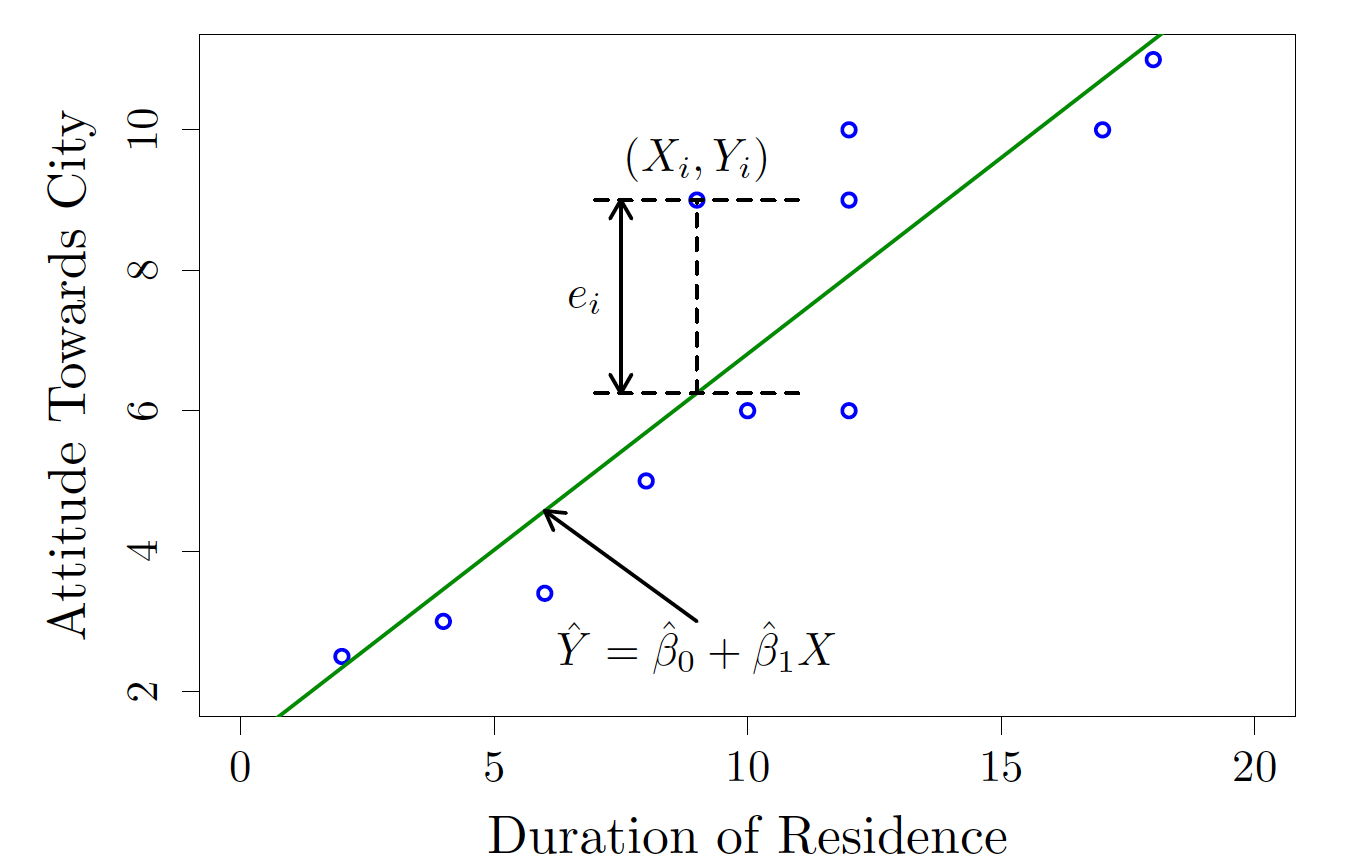
\includegraphics[width=12cm]{para3.png}
\end{frame}
\begin{frame}
	\frametitle{\textcolor{blue}{Parameter Estimation}}
	
	\begin{itemize}[label={\color{blue}$\blacktriangleright$}]
		\item We would like our estimated regression line to be as close as possible to the observations in our sample.
		
		\item That is, we want the observed values $Y_i$ to be as close as possible to the fitted values $\hat{Y}_i$.
		
		\item In other words, we want to make the residuals $e_i$ as small as we can.
	\end{itemize}
	
\end{frame}
\begin{frame}
	\frametitle{\textcolor{blue}{Parameter Estimation}}
	
	\begin{itemize}[label={\color{blue}$\blacktriangleright$}]
		\item We estimate $\beta_0$ and $\beta_1$ using the \textbf{method of least squares}.
		
		\item That is, $\hat{\beta}_0$ and $\hat{\beta}_1$ are chosen as the values that minimize the \textbf{sum of squared residuals}:
		
		\begin{align*}
			\sum_{i=1}^n e_i^2 &= \sum_{i=1}^n \left(Y_i - \hat{Y}_i\right)^2 \\[1ex]
			&= \sum_{i=1}^n \left(Y_i - \left(\hat{\beta}_0 + \hat{\beta}_1X_i\right)\right)^2
		\end{align*}
	\end{itemize}
	
\end{frame}
\begin{frame}
	\frametitle{\textcolor{blue}{Parameter Estimation}}
	
	\begin{itemize}[label={\color{blue}$\blacktriangleright$}]
		\item Using calculus, we can show that the values of $\hat{\beta}_0$ and $\hat{\beta}_1$ that minimize the sum of squared residuals are given by:
		
		\[
		\hat{\beta}_1 = \frac{s_{XY}}{s^2_X}, \qquad \hat{\beta}_0 = \bar{Y} - \hat{\beta}_1\bar{X}
		\]
		
		where $s^2_X$ is the sample variance of $X$ and $s_{XY}$ is the sample covariance between $X$ and $Y$.
	\end{itemize}
	
\end{frame}
\begin{frame}
	\frametitle{\textcolor{blue}{Parameter Estimation}}
	
	\begin{itemize}[label={\color{blue}$\blacktriangleright$}]
		\item It turns out that these estimators $\hat{\beta}_0$ and $\hat{\beta}_1$ are actually unbiased. That is:
		
		\[
		E(\hat{\beta}_0) = \beta_0, \qquad E(\hat{\beta}_1) = \beta_1
		\]
		
		\item Although we have the formulae to calculate $\hat{\beta}_0$ and $\hat{\beta}_1$, in practice we usually use a statistical software package (R, Minitab, Excel, etc) to obtain them, rather than doing it by hand.
	\end{itemize}
	
\end{frame}
\begin{frame}[fragile]
	\frametitle{\textcolor{blue}{R Output}}
	
	\begin{verbatim}
		Call:
		lm(formula = attitude ~ duration, data = city.dat)
		
		Residuals:
		Min      1Q  Median      3Q     Max 
		-1.9262 -0.7640 -0.4579  0.6165  2.7494 
		
		Coefficients:
		Estimate Std. Error t value Pr(>|t|)
		(Intercept)   1.2237     1.0531   1.162 0.275114
		duration      0.5585     0.0952   5.867 0.000239
		
		Residual standard error: 1.493 on 9 degrees of freedom
		Multiple R-squared: 0.7927,    Adjusted R-squared: 0.7697
		F-statistic: 34.42 on 1 and 9 DF,  p-value: 0.0002387
	\end{verbatim}
	
\end{frame}
\begin{frame}
	\frametitle{\textcolor{blue}{Assessing the Model}}
	
	\begin{itemize}[label={\color{blue}$\blacktriangleright$}]
		\item So we have defined the simple linear regression model and we know how to fit (or estimate) the model.
		
		\item The next important step is to \textit{assess} our simple linear regression model.
		
		\item In other words, we want to determine whether or not the model is any good.
	\end{itemize}
	
\end{frame}
\begin{frame}
	\frametitle{\textcolor{blue}{Assessing the Model}}
	
	\begin{itemize}[label={\color{blue}$\blacktriangleright$}]
		\item There are a number of things we can do in order to assess our simple linear regression model:
	\end{itemize}
	
	\begin{enumerate}[label={\color{blue}\arabic{enumi}}.]
		\item Check to see if the model assumptions hold.
		\item Test the overall significance of the model.
		\item Estimate $\sigma_\epsilon^2$, the variance of the error variable.
		\item Calculate $R^2$, the proportion of variation in $Y$ explained by the model.
	\end{enumerate}
	
\end{frame}
\begin{frame}
	\frametitle{\textcolor{blue}{1. Checking the Model Assumptions}}
	
	\begin{itemize}[label={\color{blue}$\blacktriangleright$}]
		\item The first thing we should do after fitting the model is to check if the model assumptions hold.
		
		\item If they do not hold, it means that a simple linear regression model is not appropriate for our data.
		
		\item Recall that the model assumptions were stated in terms of the error variable, namely, $\epsilon_i \stackrel{iid}{\sim} N(0, \sigma_\epsilon^2)$.
		
		\item We don't know the true errors $\epsilon_i$, but we do know the residuals $e_i = Y_i - \hat{Y}_i$, which estimate the true errors.
	\end{itemize}
	
\end{frame}
\begin{frame}
	\frametitle{\textcolor{blue}{1. Checking the Model Assumptions}}
	\centering
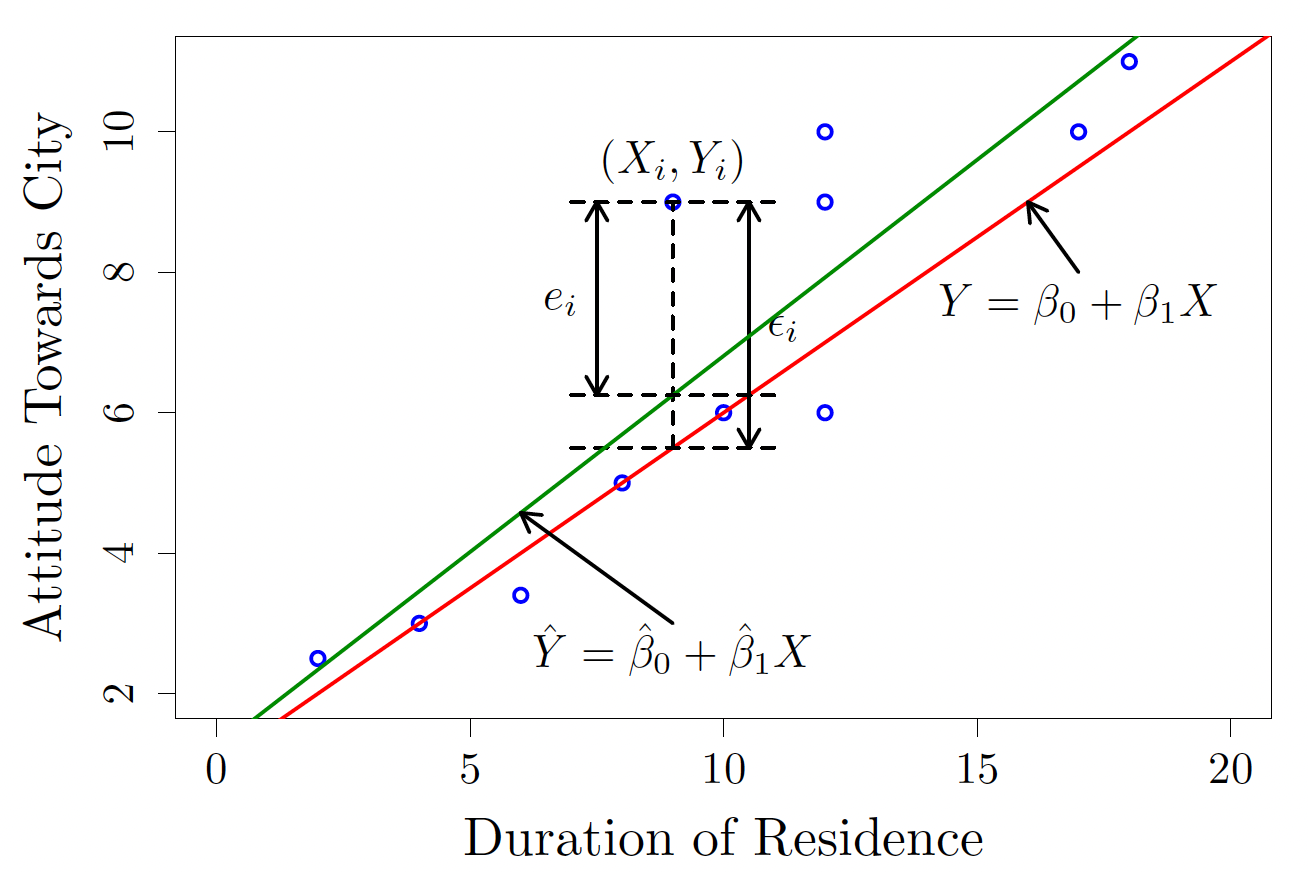
\includegraphics[width=12cm]{check.png}
\end{frame}
\begin{frame}
	\frametitle{\textcolor{blue}{1. Checking the Model Assumptions}}
	
	\begin{itemize}[label={\color{blue}$\blacktriangleright$}]
		\item So we should check to see if the residuals $e_i$ satisfy the model assumptions:
		\begin{enumerate}
			\item[\textcolor{blue}{(a)}] Are they normally distributed?
			\item[\textcolor{blue}{(b)}] Do they have mean 0 and constant variance?
			\item[\textcolor{blue}{(c)}] Are they independent?
		\end{enumerate}
		
		\item[\textcolor{blue}{(a)}] To check the normality of the residuals, we can generate:
		\begin{itemize}[label={\color{blue}$\blacktriangleright$}]
			\item A histogram of the residuals, which should look like a normal distribution (bell-shaped and symmetric).
			\item A normal probability plot of the residuals, which should be linear.
		\end{itemize}
	\end{itemize}
	
\end{frame}
\begin{frame}
	\frametitle{\textcolor{blue}{1. Checking the Model Assumptions}}
	
	\begin{itemize}
		\item[\textcolor{blue}{(b)}] To check that the residuals have mean 0 and constant variance, we can examine scatter plots of the residuals against the $X$ values or fitted values.
		\begin{itemize}[label={\color{blue}$\blacktriangleright$}]
			\item These \textit{residual plots} should look like a random scatter of points about 0 with no obvious patterns or trends.
			\item If there are clear patterns or trends, we might need to transform the data.
		\end{itemize}
	\end{itemize}
	
\end{frame}
\begin{frame}
	\frametitle{\textcolor{blue}{A Good Residual Plot}}
	\centering
	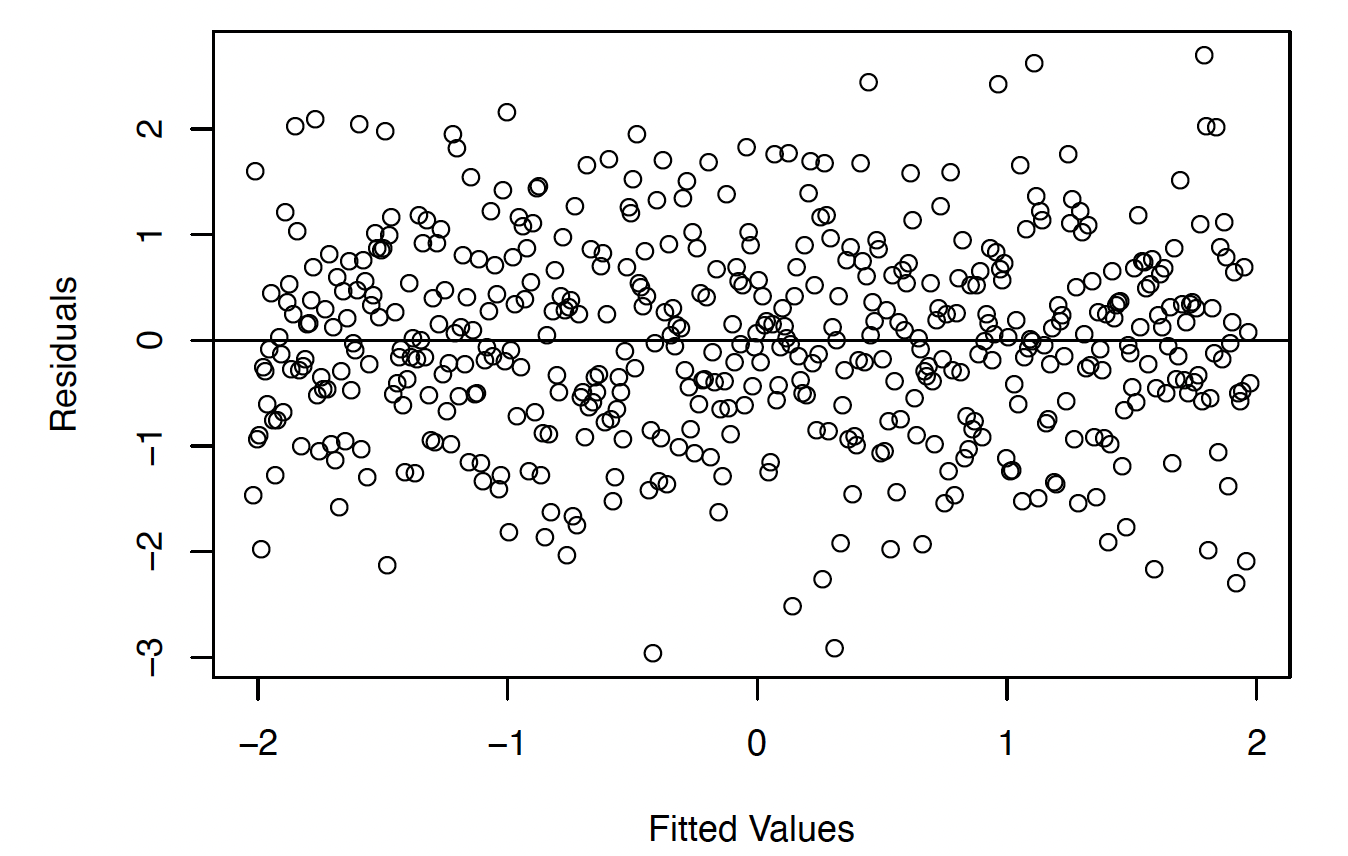
\includegraphics[width=12cm]{goodresi.png}
\end{frame}
\begin{frame}
	\frametitle{\textcolor{blue}{A Bad Residual Plot}}
	\centering
	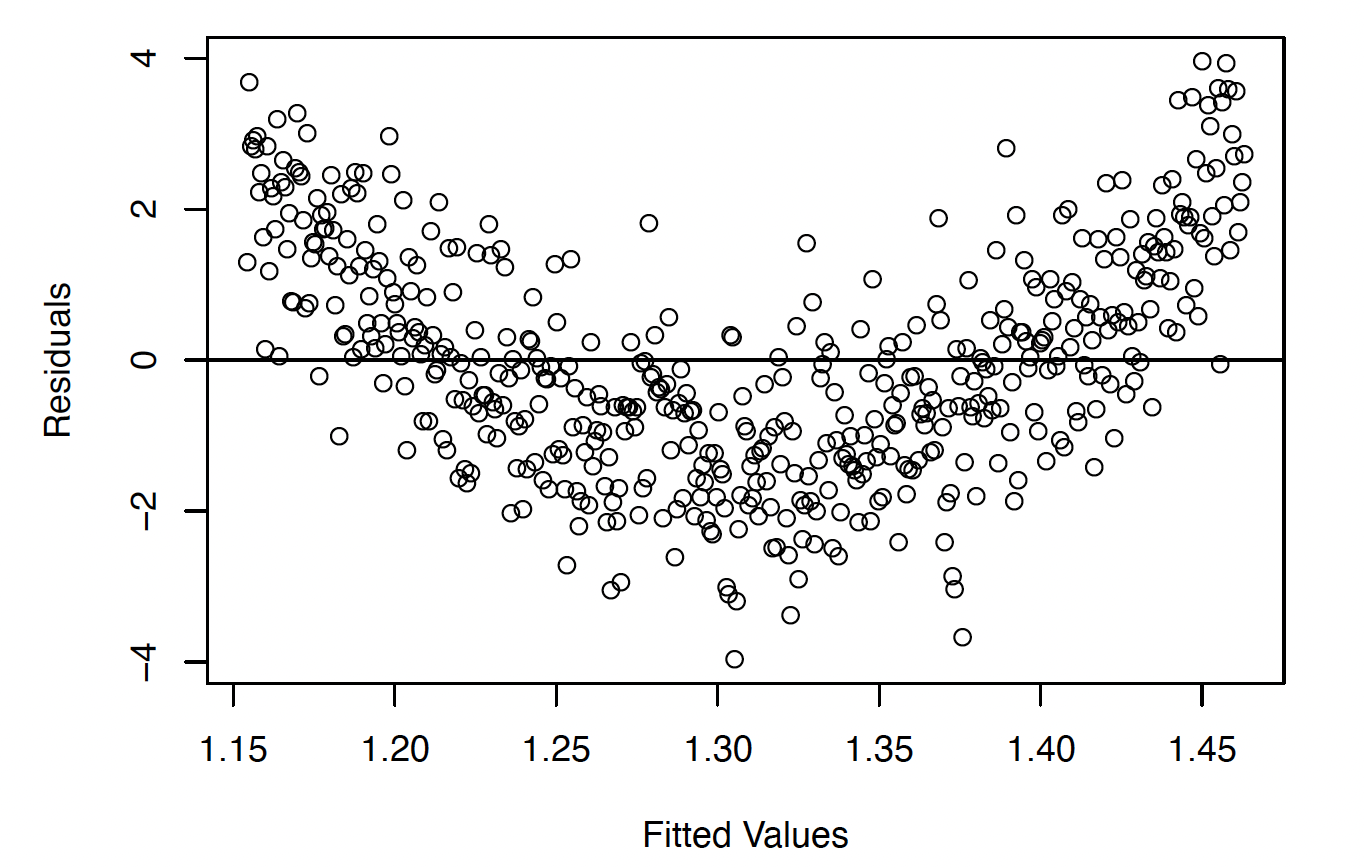
\includegraphics[width=12cm]{bad.png}
\end{frame}
\begin{frame}
	\frametitle{\textcolor{blue}{Another Bad Residual Plot}}
	\centering
	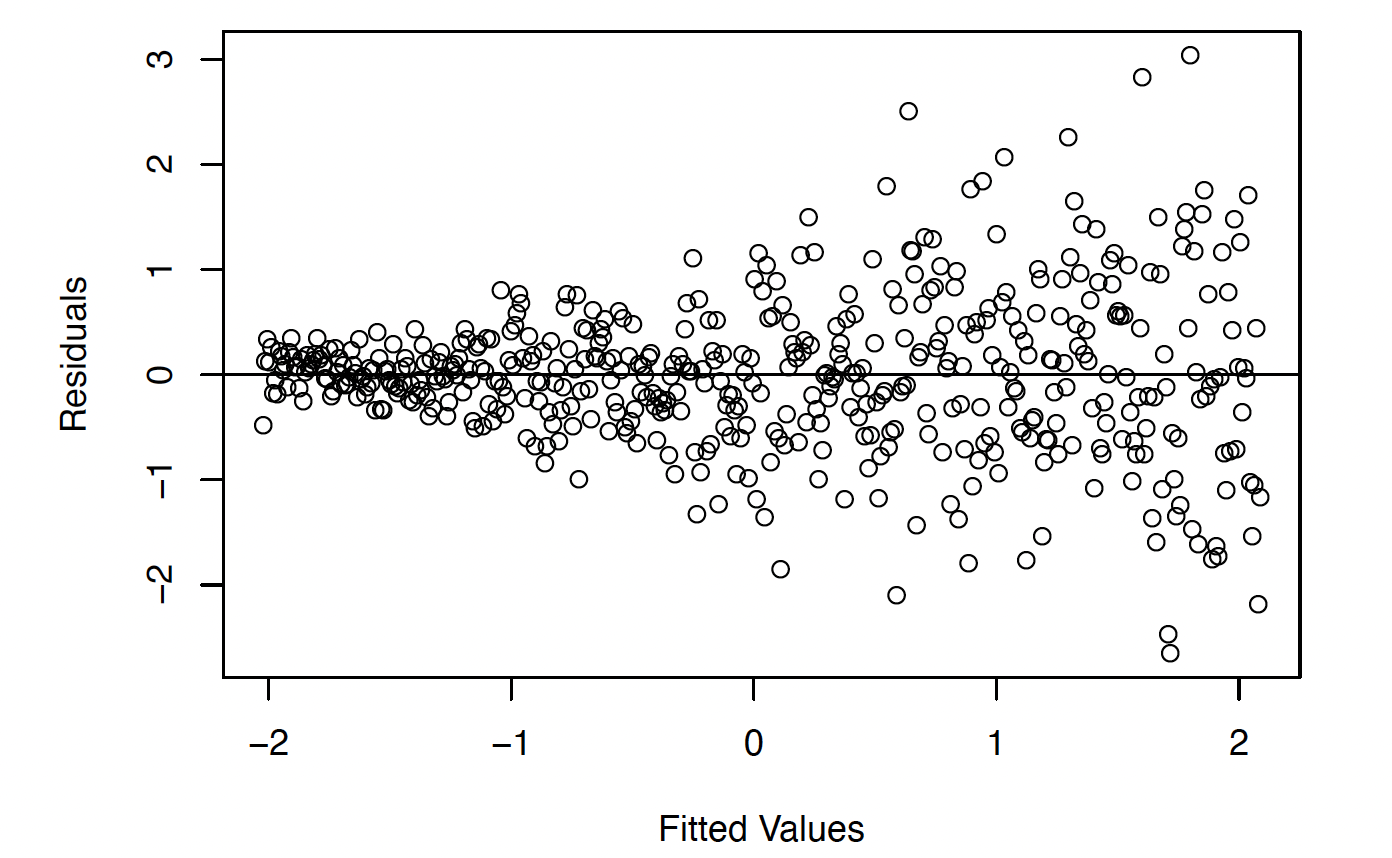
\includegraphics[width=12cm]{abad.png}
\end{frame}
\begin{frame}
	\frametitle{\textcolor{blue}{1. Checking the Model Assumptions}}
	
	\begin{itemize}
		\item[\textcolor{blue}{(c)}] Certain plots can be used for checking the independence of the residuals, but if the sample is collected properly (i.e., randomly) this hopefully shouldn't be a major problem.
		\begin{itemize}[label={\color{blue}$\blacktriangleright$}]
			\item Can plot the residuals against the order in which the observations were collected to see if there is any time correlation between the residuals.
		\end{itemize}
	\end{itemize}
	
\end{frame}
\end{document}